%% ==============================
\chapter{State of the art}
\label{sec:state_of_the_art}
%% ==============================
Questions to ask:
\begin{enumerate}
    \item What is generally known about the topic? (relevant theory)
    \item What are the most important (recent) existing works in the field related to the research problem? 
    \item Provide a comprehensive review of the relevant literature, including key theories, concepts, and previous studies that inform your research question.
    \item What are the limitations or gaps in the existing works that this work aims to address? 
    \item How does this work build upon or differ from existing works? 
    \item What are the main research approaches or techniques used in the field, and how do they relate to this work? 
    \item What are the main challenges or open questions in the field? 
\end{enumerate}

General theory:
\begin{enumerate}
    \item Path planning
    \item Astar, RRT, Dijkstra, PRM
    \item Hierarchical graphs
    \item ROS2 Nav Stack
    \item OpenRMF
    \item Behavior Trees
\end{enumerate}

The following overview of the state of the art consist of four main parts:
\begin{enumerate}
    \item The general theory of path planning in mobile robotics is presented. This includes the most common algorithms for path planning, and their applications in real robotic systems. (Chapter \ref{sec:path_planning}).
    \item The recent approaches to hierarchical path planning in complex multi-floor environments are presented. This shows the existing approaches to the first research question: "How to navigate in complex multi-floor environments?" (Chapter \ref{sec:hierarchical_planning}).
    \item The recent approaches to straight path planning are presented. This shows the existing approaches to the second research question: "How to plan paths that are straight and human-predictable?" (Chapter \ref{sec:straight_paths}).
    \item The research gap and limitations of the state of the art is summarized in Chapter \ref{sec:research_gap}.
\end{enumerate}

%% ==============================
\section{General Path Planning for Mobile Robots}
\label{sec:path_planning}
%% ==============================

The general approach to path planning in mobile robotics is a two-layered architecture which can be seen in Figure \ref{fig:path_planning_two_layered_architecture}. The first layer is the global path planning layer. It is responsible for finding a path from the start to the goal position in a previously known static environment. The second layer is the collision avoidance also known as local path planner or controller. It is responsible for avoiding dynamic obstacles that prevent the global path from being executed. For both layers there are different approaches as open source solutions available. This concept is further explained with the example in chapter \ref{sec:navigation_stack}.

\begin{figure}[h]
    \centering
    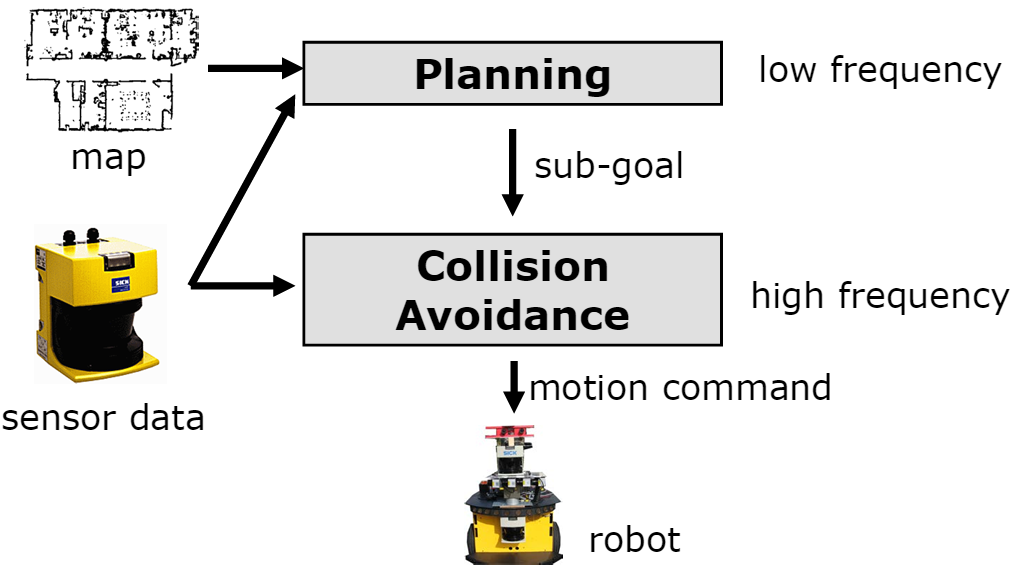
\includegraphics[width=0.75\textwidth]{figures/20_state_of_the_art/path_planning_two_layered_architecture.png}
    \caption[The two layered architecture for mobile robot path planning]{The two layered architecture for mobile robot path planning (Source: \cite{burgard_introduction_2021})}
    \label{fig:path_planning_two_layered_architecture}
\end{figure}
The scope of this work is limited to extending the capabilities of the global planner for multiple floors. The collision avoidance is solved with existing algorithms. The following sections will give an overview of the most common existing global planner algorithms. 



%% ==============================
\subsection{Path Planning Algorithms}
Planning a path is a major challenge in robotics and is necessary for mobility. The path from the robot's current location to the goal can be planned in two ways: deterministically or probabilistically. Deterministic planners use algorithms that always deliver the same results with the same input. Probabilistic planners, on the other hand, are based on randomness and produce different results for the same input. The map on which deterministic planners are based is usually discretised into a lattice. In an informed search, heuristics can be used to tell whether one grid field is closer to the target configuration than another. According to Burgard \cite{burgard_introduction_2021}, the performance of a search algorithm is measured in four different ways:
\begin{enumerate}
    \item Completeness:
    Does the algorithm find a solution when there is one?
    \item Optimality:
    Is the solution the best one of all possible solutions in terms of path cost?
    \item Time complexity:
    How long does it take to find a solution?
    \item Space complexity:
    How much memory is needed to perform the search?
\end{enumerate}

Among the deterministic planners there are various prominent representatives, such as the Dijkstra or the A* algorithm as a special form of it. The A* was originally proposed by Hart, Nilsson and Raphael \cite{hart_formal_1968} and is frequently used in research. A* plans a path from the start configuration to the target configuration. During expansion, every new node is evaluated with the metric \ref{equ:metric}. 
\begin{equation} \label{equ:metric}
    f(n) = g(n) + h(n)
\end{equation}
The node with the lowest metric score is expanded next. The metric consists of the cost of the previously traveled path \(g(n)\) up to the current node \(n\) added with the estimated cost of the remaining path to the goal \(h(n)\). This estimation is calculated with a heuristic like the euclidean distance or Manhattan distance for gridmaps. It is important that the heuristic never over-estimates the real costs to ensure the optimality of the A* algorithm. In planar 2D space there is no path shorter than the direct line with length of the euclidean distance. The expansion is done until the goal node is part of the expanded nodes. The shortest path is then traced back by following the parent nodes until the start.

The Dijkstra algorithm \cite{dijkstra_note_1959} is a generalizied form of the A* and only considers the previous costs \(g(n)\) during expansion. In general this leads to more nodes beeing searched and a longer search time for the goal than A*. The time and space complexity of Dijkstra are higher than for A*. Both algorithms have the advantage of providing complete and optimal solutions.

\begin{figure}[h]
    \centering
    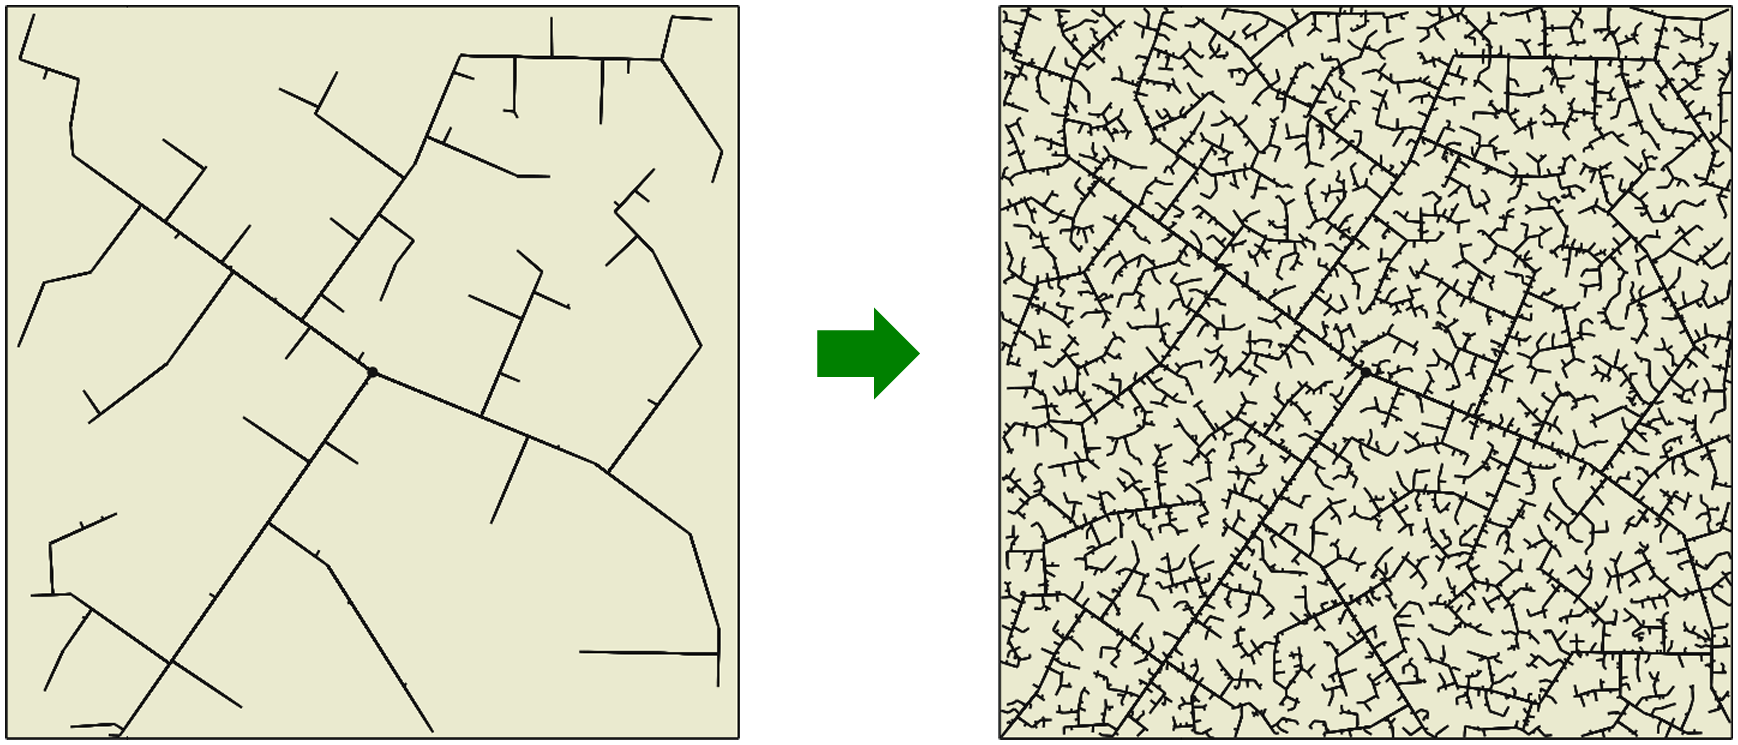
\includegraphics[width=1\textwidth]{figures/20_state_of_the_art/rrt.png}
    \caption[The RRT algorithm]{Rapidly-exploring Random Tree (RRT) after 45 (left) and 2345 (right) iterations from the start node in each center. (Source: \cite{burgard_introduction_2021})}
    \label{fig:rrt}
\end{figure}

In contrast to deterministic planners, probabilistic planners are based on the principle of chance. One example of many is the RRT. New nodes are randomly selected in the search field, then an attempt is made to connect these with the closest node, which is already part of the tree. This connections has to satisfy two conditions: First there is no obstacle in the direct connection line and second the distance to the tree is not bigger than \(d_{max}\). If the first criterion fails, the selected node is discarded. If only the second criterion fails, a new node is created on the connecting line with the distance \(d_{max}\) and added to the tree. This procedure creates large trees after only a few iterations, as can be seen in Figure 2.3. With an appropriately chosen \(d_{max}\), this method needs significantly fewer nodes to reach the goal than an A*. In addition with the number of nodes approaching infinity, this algorithm also moves in the direction of completeness, but this method is not optimal. Time and memory complexity are dependent on \(d_{max}\).


%% ==============================
\subsection{The Robot Operating System 2}
\begin{displayquote}
    \enquote{The \acrfull{ros} is a framework for writing robot software. It is a collection of tools, libraries, and conventions that aim to simplify the task of creating
    complex and robust robot behavior across a wide variety of robotic platforms.} \cite{quigley_programming_2015}
\end{displayquote}
    
\begin{figure}[h]
    \centering
    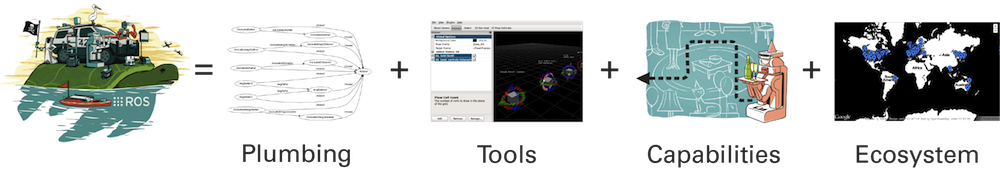
\includegraphics[width=1\textwidth]{figures/20_state_of_the_art/ros_equation.png}
    \caption[The ROS equation]{The ROS equation: ROS = Plumbing + Tools + Capabilities + Community (Source: \cite{open_robotics_ros_2020})}
    \label{fig:ros_equation}
\end{figure}

The development of \gls{ros} began in 2007 as part of the Stanford AI Robot Project (STAIR) and was mainly driven by Willow Garage. There it was used as the basis for the Personal Robot 2 (PR2), but has been intended from the start as an open-source platform for a wide range of robotic applications. By now, the development is being driven forward by Open Robotics. The founders, Brian Gerkey and Morgan Quigley, have also published a comprehensive book to make it easier to get started with \gls{ros} \cite{quigley_programming_2015}. The \gls{ros} ecosystem consists of much more than pure code; it thrives on a large community and the exchange of ready-to-use packages, which is described by the '\gls{ros} equation' in Figure \ref{fig:ros_equation}. Since 2011, \gls{ros} has has left the earth for the International Space Station with NASA's Robonaut 2 \cite{koubaa_ros_2016}. Due to the rapidly growing community and increasing application in industry, an improved version was developed and released in December 2018 as \gls{ros_2}. The main difference is the focus on real-time applications and the use of the industry standard 'Data Distribution Service' (DDS) for the communication of distributed systems \cite{macenski_robot_2022}.

Nodes are the basis of the distributed network of an \gls{ros} application. The nodes are executed independently of each other and communicate with each other via defined interfaces. This offers the advantage that applications can be built up modular, can be easily exchanged, and can be used in conjunction with other applications. A node can contain several topics, services or actions with which data can be exchanged with other nodes. Different nodes in a \gls{ros} application can be executed on different hardware. A collection of nodes that perform a completed function are grouped together as a package and shared by many developers around the world. A combination of related packages with a version history and managed documentation is called a stack. For example, there is the Navigation Stack, which contains all the functions needed to move the robot safely from A to B. This includes algorithms for localisation and path planning as well as the processing of sensor data for obstacle avoidance and mapping.

\begin{figure}[h]
    \centering
    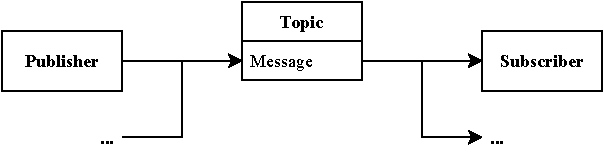
\includegraphics[width=0.75\textwidth]{figures/20_state_of_the_art/topics.pdf}
    \caption{The structure of a ROS topic}
    \label{fig:topics}
\end{figure}

The individual nodes communicate through message channels about a specific topic. This communication is designed for distributed systems and enables a many-to-many (n:m) cardinality. This means that each node can act as a publisher or subscriber of any topic, see Figure \ref{fig:topics}. The content of the message is defined by a .msg file as the interface.

\begin{figure}[h]
    \centering
    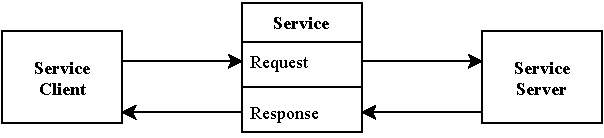
\includegraphics[width=0.75\textwidth]{figures/20_state_of_the_art/services.pdf}
    \caption{The structure of a ROS service}
    \label{fig:services}
\end{figure}

Services are based on the call-and-response model. This means that, unlike topics, messages are not unilaterally sent into the network. Instead, a request is made from a client to a server, and a response is sent back, as illustrated in Figure \ref{fig:services}. The structure resembles a function call, where parameters are passed and a return value is expected. The data types are defined in the corresponding .srv file. This type of communication is particularly useful for computations performed by another node \cite[p. 51]{quigley_programming_2015}. Services can be executed synchronously or asynchronously. In a synchronous call, the calling node blocks the thread until the response arrives. Synchronous calls should only be used when the service requires a short, finite amount of time for computation. Asynchronous calls are implemented by providing a predefined function (callback) that is automatically invoked by \gls{ros} when the service response is received. This allows other code to be executed in the node as long as it does not depend on the service result.

\begin{figure}[h]
    \centering
    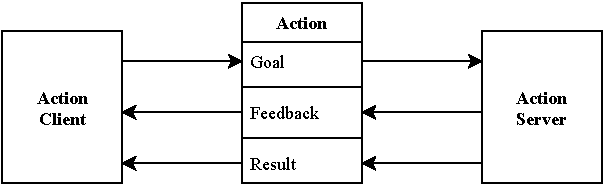
\includegraphics[width=0.75\textwidth]{figures/20_state_of_the_art/actions.pdf}
    \caption{The structure of a ROS action}
    \label{fig:actions}
\end{figure}

Actions have been a fixed component of the communication vocabulary since \gls{ros_2}. They are designed for the asynchronous execution of long-duration actions. In addition to the concept of services, actions allow for the exchange of feedback data during execution. Furthermore, actions provide the ability to cancel their execution. An action client sends a request (goal) to the action server, which can either accept or reject the goal. During execution, a feedback callback is invoked at the client until the result is received and processed. Actions offer a high-level communication protocol, as shown in Figure \ref{fig:actions}. A good example of the application of actions is robot movement towards a specific goal. The task should occur asynchronously and can vary in duration. Through the feedback mechanism, information about the current position of the robot can be communicated, and if the goal becomes outdated, the action can be canceled. The interface of an action for navigation is defined by an .action file, as depicted in Algorithm \ref{lst:navigatetopose.action}.

\lstset{language=python, caption={NavigateToPose.action, definition of an action from type 'NavigateToPose'}, label={lst:navigatetopose.action}}
\begin{lstlisting}
# goal
geometry_msgs/PoseStamped pose
-%{}%-%{}%-
# result
std_msgs/Empty result
-%{}%-%{}%-
# feedback
geometry_msgs/PoseStamped current_pose
builtin_interfaces/Duration navigation_time
int16 number_of_recoveries
float32 distance_remaining
\end{lstlisting}
    
%% ==============================
\subsection{The Navigation Stack in ROS2}
\label{sec:navigation_stack}

\begin{displayquote}
    \enquote{Nav2 is the professionally supported spiritual successor of the ROS Navigation Stack. This project seeks to find a safe way to have a mobile robot move to complete complex tasks through many types of environments and classes of robot kinematics. Not only can it move from Point A to Point B, but it can have intermediary poses, and represent other types of tasks like object following and more. Nav2 is a production-grade and high-quality navigation framework trusted by 50+ companies worldwide.} \cite{steve_macenski_navigation_2020}
\end{displayquote}

The \gls{nav_2} stack for \gls{ros_2} is a comprehensive framework for the development of new planner algorithms. The planner developed in this work is based on the \gls{nav_2} stack and is written as an exchangeable plugin for the existing structure. With its server and plugin layout \gls{nav_2} supports custom planner, controller behavior and smoother plugins. In Figure \ref{fig:nav2_architecture} the architecture of \gls{nav_2} is shown. It follows the classic two-layered architecture for path planning seen in Figure \ref{fig:path_planning_two_layered_architecture}. The planner server provides the global path planning on a known map and the controller server offers algorithms for following this path with dynamic obstacle avoidance. The necessary inputs for this system are the map, the odometry of the robot wheels and the sensor data from lidars or cameras. With this information the localization can calculate the most likely position of the robot in the map. The planner plans a path from this current position to the goal. In a control loop, the controller tries to reduce the error between the current position and the planned path. The output of the controller is a velocity command for the robot. The velocity command is then executed by the robot's motor controller.

\begin{figure}[h]
    \centering
    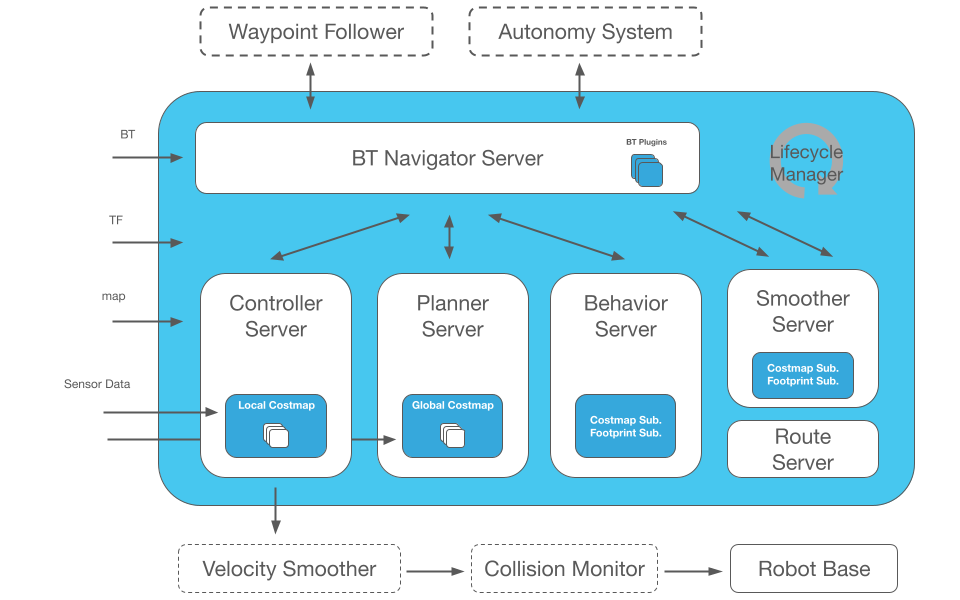
\includegraphics[width=\textwidth]{figures/20_state_of_the_art/nav2_architecture.png}
    \caption[The architecture of the \gls{nav_2} stack]{The architecture of the \gls{nav_2} stack (Source: \cite{steve_macenski_navigation_2020})}
    \label{fig:nav2_architecture}
\end{figure}

In this work a new planner, capable of planning in complex multi-floor environments, is developed. The algorithm is implemented as a plugin for the planner server. The rest of the \gls{nav_2} pipeline is used with existing packages.

%% ==============================
\subsection{Behavior Trees for Navigation}

\gls{nav_2} is the most prominent example of \glspl{bt} in robotics and especially for navigation. It uses \glspl{bt} to create customized and intelligent navigation behavior by orchestrating many independent modular servers. The default \gls{bt} for executing a navigation request to a specific goal is shown in Figure \ref{fig:nav2_bt}. It shows the actual planner, an A* algorithm, on the left side which is triggered every second (1 Hz). All other named actions are recovery behaviors which are used to clear the costmaps and reorient the robot if it gets stuck. To understand the symbolic language of the \gls{bt} the single elements are explained in the following section.

\begin{figure}[h]
    \centering
    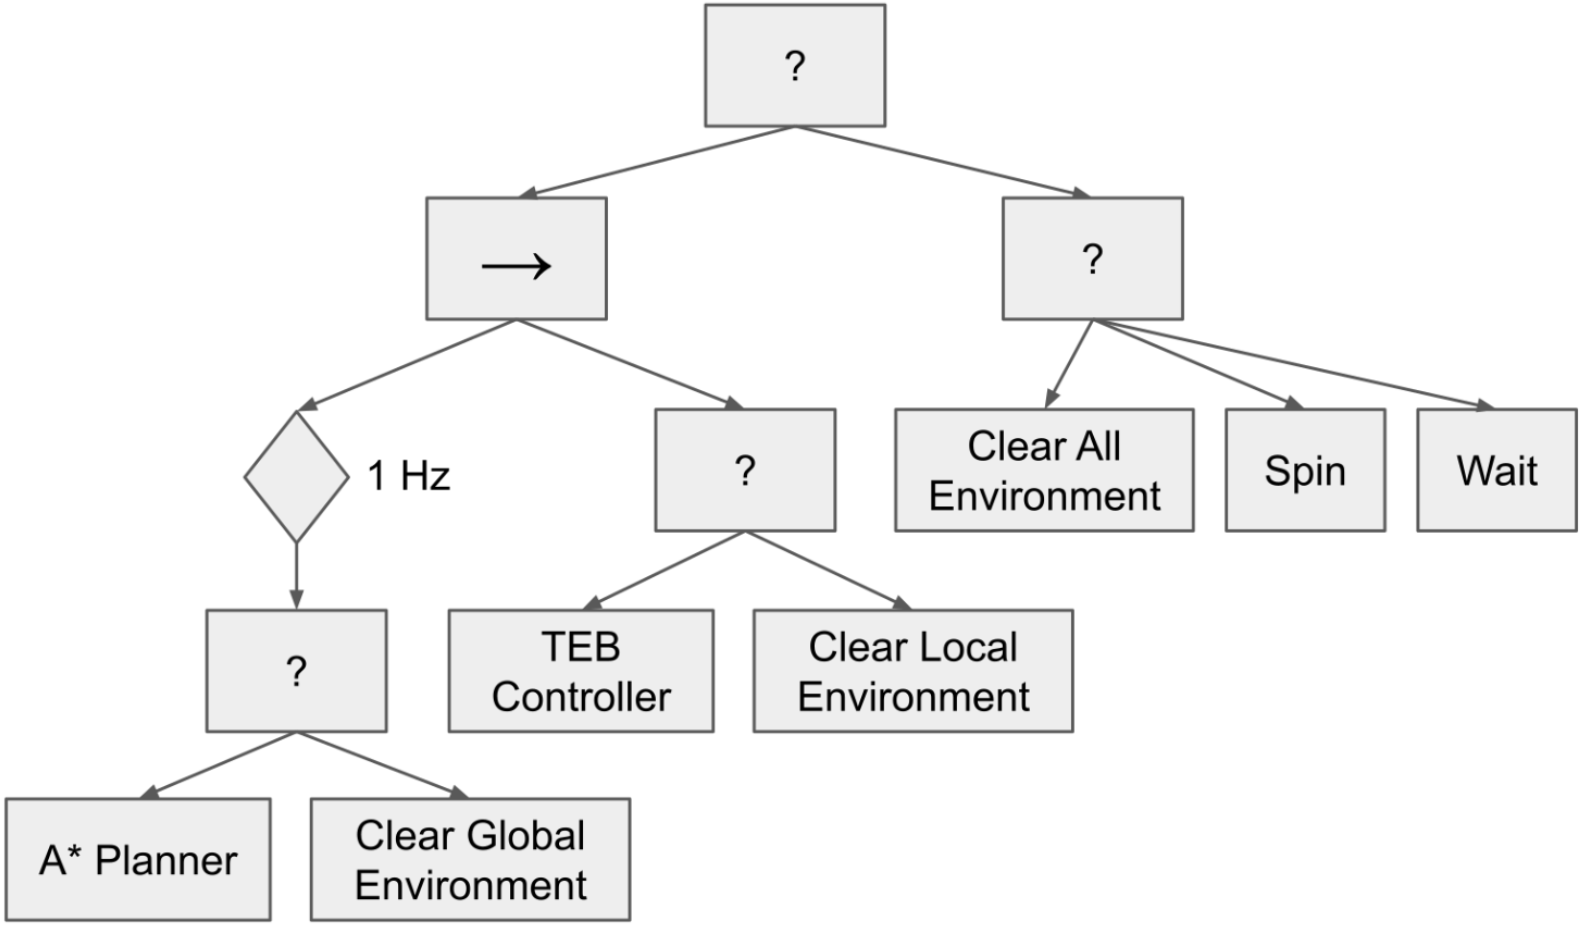
\includegraphics[width=\textwidth]{figures/20_state_of_the_art/nav2_bt.png}
    \caption[The default navigation behavior]{The default navigation behavior (Source: \cite{macenski_marathon_2020})}
    \label{fig:nav2_bt}
\end{figure}

\Glspl{bt} were developed for video games to describe the behavior of computer-controlled characters in a modular way \cite{hutchison_evolving_2010}. \Glspl{bt} combine a deliberative approach with reactive components. The internal structure of the tree establishes an overall plan of actions, ensuring goal-oriented behavior. However, reactive behavior can still be triggered through constant reevaluation of all conditions. 

A \gls{bt} consists of small building blocks that can be combined to create any control structure. The biggest difference from State Machines is that in \glspl{fsm}, a state-dependent transition is triggered after a specific input. In \glspl{bt}, on the other hand, the entire structure is updated at regular, short time intervals, and all conditions are re-evaluated. This allows for arbitrary transitions to occur based on the appropriate preconditions, without explicitly defining them.

The fundamental element of every \gls{bt} is the root node, from which the attached nodes are updated (ticked). Each node returns either Success, Failure, or Running after being updated. In general, a \gls{bt} can be described using an \gls{fsm}, where the state transitions can take three possible states into account, as shown in Figure \ref{fig:fsm_general_bt}.

\begin{figure}[h]
    \centering
    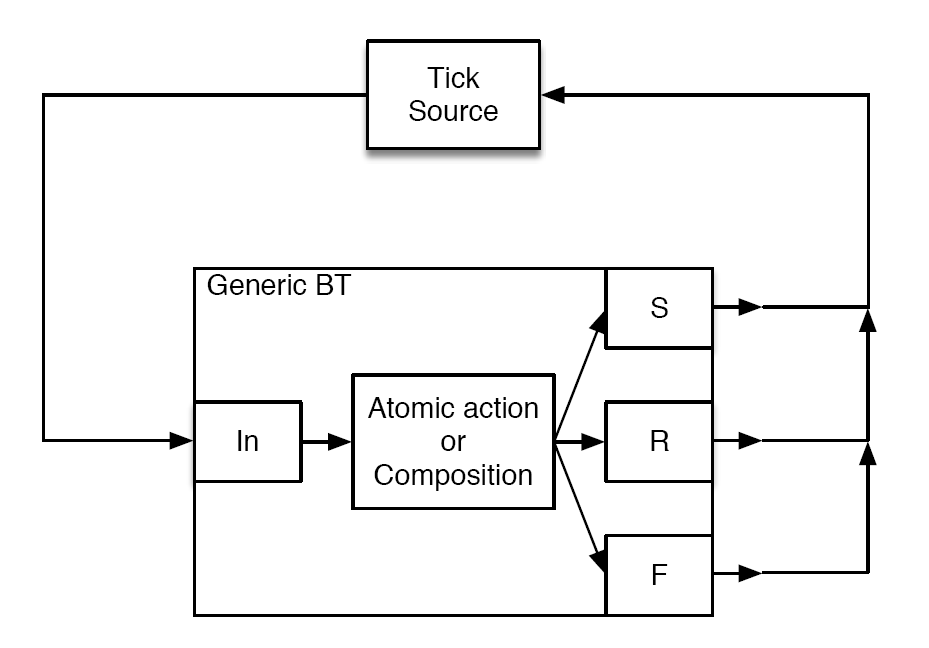
\includegraphics[width=0.7\textwidth]{figures/20_state_of_the_art/fsm_general_bt.png}
    \caption[General \gls{bt} displayed as \gls{fsm}]{General \gls{bt} displayed as \gls{fsm} with the state transitions: Success (S), Running (R) and Failure (F) (Source: \cite{colledanchise_behavior_2018})}
    \label{fig:fsm_general_bt}
\end{figure}

The basic building blocks of a \gls{bt} are shown in Figure \ref{fig:bt_types}. Actions represent individual, self-contained algorithms that execute specific commands to actuators or perform calculations. An Action can run in a blocking (synchronous) manner, where it returns either Success or Failure after its start, or it can run asynchronously and maintain a Running state during execution. Conditions, on the other hand, take either Success or Failure states depending on the condition being evaluated.

\begin{figure}[h]
    \centering
    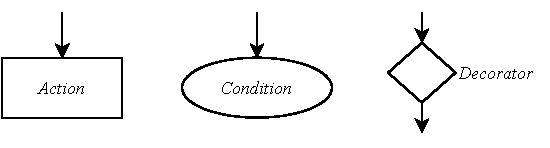
\includegraphics[width=0.7\textwidth]{figures/20_state_of_the_art/bt_types.pdf}
    \caption{Graphical representation of Actions, Conditions and Decorators}
    \label{fig:bt_types}
\end{figure}

The Decorator is a type of control node that has only one child. It allows the state of the child node to be influenced by custom-defined rules, avoiding complex constructions with Sequences and Fallbacks. Examples of Decorators include Inverters, Time Delays, and Repeaters (repeating a certain number of times or until a successful completion).

\begin{figure}[h]
    \centering
    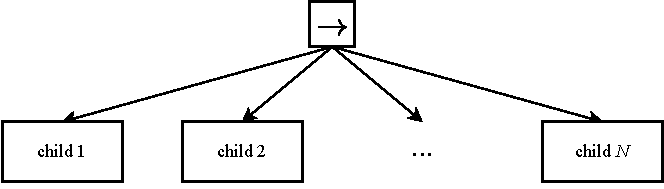
\includegraphics[width=0.75\textwidth]{figures/20_state_of_the_art/sequence.pdf}
    \caption{Graphical BT of a Sequence with \textit{N} childs}
    \label{fig:sequence}
\end{figure}

\lstset{language=C++, caption={Algorithm of a Sequence with \textit{N} childs}, label={lst:pseudo_code_sequence}, morekeywords={from, to}}
\begin{lstlisting}[float=h]
for i from 1 to %\textit{N}% do
    child_status = tick(child[i])
    
    if child_status == %\textit{Running}%
        return %\textit{Running}%
        
    if child_status == %\textit{Failure}%
        return %\textit{Failure}%

return %\textit{Success}%
\end{lstlisting}

The Sequence starts its children from left to right in the graphical representation, as shown in Figure \ref{fig:sequence}. If a child returns Running, the entire Sequence is considered Running. Upon successful execution of a child, the next child is started, continuing until all children, and thus the entire Sequence, achieve the Success state. If a child cannot be executed successfully, the loop is aborted, and the Sequence enters the Failure state, as shown in Algorithm \ref{lst:pseudo_code_sequence}.
  

\begin{figure}[h]
    \centering
    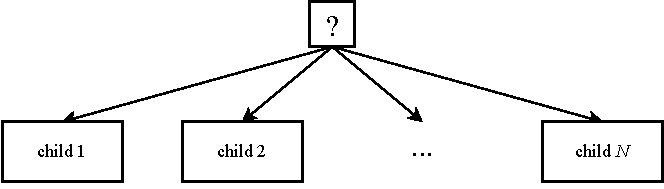
\includegraphics[width=0.75\textwidth]{figures/20_state_of_the_art/fallback.pdf}
    \caption{Graphical BT of a Fallback with \textit{N} childs}
    \label{fig:fallback}
  \end{figure}
  
  \lstset{language=C++, caption={Algorithm of a Fallback with \textit{N} childs}, label={lst:pseudo_code_fallback}, morekeywords={from, to}}
  \begin{lstlisting}[float=h]
  for i from 1 to %\textit{N}% do
      child_status = tick(child[i])
      
      if child_status == %\textit{Running}%
          return %\textit{Running}%
          
      if child_status == %\textit{Success}%
          return %\textit{Success}%
  
  return %\textit{Failure}%
  \end{lstlisting}

  A Fallback node (also known as Selector) executes only one child successfully, unlike the Sequence. All children are updated from left to right, as shown in Figure \ref{fig:fallback} and Algorithm \ref{lst:pseudo_code_fallback}. Once a child reaches the Success state, the Fallback is completed. If a child returns Failure, the next child is started.

\begin{figure}[h]
    \centering
    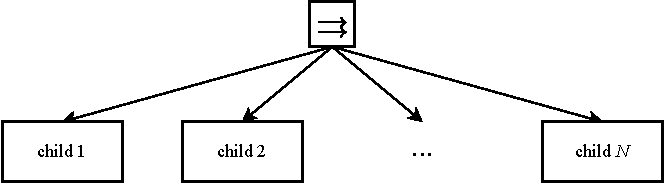
\includegraphics[width=0.75\textwidth]{figures/20_state_of_the_art/parallel.pdf}
    \caption{Graphical BT of a Parallel with \textit{N} childs}
    \label{fig:parallel}
\end{figure}
  
\lstset{language=C++, caption={Algorithm of a Parallel with \textit{N} childs and success count \textit{M}}, label={lst:pseudo_code_parallel}, morekeywords={from, to}}
\begin{lstlisting}[float=h]
for i from 1 to %\textit{N}% do
    child_status[i] = tick(child[i])
    
if success_count(child_status) >= %\textit{M}%
    return %\textit{Success}%
        
if failure_count(child_status) > (%\textit{N}% - %\textit{M}%)
    return %\textit{Failure}%

return %\textit{Running}%
\end{lstlisting}

In addition to the control nodes Sequence and Fallback, there is also the Parallel node. In this structure, all children are started simultaneously, and the final state of the Parallel node is determined based on a comparison between a defined count M and the number of successfully completed children, as shown in Figure \ref{fig:parallel} and Algorithm \ref{lst:pseudo_code_parallel}.

An overview of the functions of each element is presented in Table \ref{tab:overview_bt}.

\begin{table}[h]
\centering
\resizebox{\textwidth}{!}{%
%\setlength{\extrarowheight}{8pt}
\begin{tabular}{lclll}
\toprule
\textbf{} & \multicolumn{1}{l}{\textbf{}} & \multicolumn{3}{c}{\textbf{Return Status}} \\ \midrule
\multicolumn{1}{c}{\textbf{Type}} & \textbf{Symbol} & \multicolumn{1}{c}{\textbf{Success}} & \multicolumn{1}{c}{\textbf{Failure}} & \multicolumn{1}{c}{\textbf{Running}} \\ \midrule
\textbf{Action} & Text & When completed & In case of errors & During execution \vspace{3mm}\\
\textbf{Condition} & Text & When condition is true & When condition is false & Never \vspace{3mm}\\
\textbf{Sequence} & $\to$ & When all children are \textit{Success} & When a child is \textit{Failure} & When a child is \textit{Running} \vspace{3mm}\\
\textbf{Fallback} & ? & When a child is \textit{Success} & When all children are \textit{Failure} & When a child is \textit{Running} \vspace{3mm}\\
\textbf{Parallel} & $\rightrightarrows$ & \begin{tabular}[c]{@{}l@{}}When $\ge$ \textit{M} \\ children are \textit{Success}\end{tabular} & \begin{tabular}[c]{@{}l@{}}When > \textit{N} - \textit{M} \\ children are \textit{Failure}\end{tabular} & \begin{tabular}[c]{@{}l@{}}As long as limits \\ are not reached\end{tabular} \vspace{3mm}\\
\textbf{Decorator} & $\diamond$ & Depending on the function & Depending on the function & Depending on the function \\ \bottomrule
\end{tabular}%
}
\caption{Overview of the elements of a Behavior Tree}
\label{tab:overview_bt}
\end{table}

\Glspl{bt} represent an evolution of \gls{fsm}, which are still widely used, but offer several advantages beyond them. The following are the advantages and drawbacks of \glspl{bt}. These characteristics are not necessarily unique to \glspl{bt} but also apply to other concepts such as \glspl{hfsm} or decision trees \cite{colledanchise_behavior_2018}.

\begin{enumerate}
  \item \textbf{Modularity:} Individual subsystems can be modified and replaced as needed. The entire BT can also be reused as a module.
  \item \textbf{Hierarchical Structure:} Each control node introduces an additional level of hierarchy, making the overall behavior easier to understand.
  \item \textbf{Reusability:} Defined interfaces allow code to be used in multiple locations.
  \item \textbf{Reactiveness:} By continuously updating the BT, actions can be executed in a closed loop, enabling dynamic responses to the environment.
  \item \textbf{Intuitive Representation:} The graphical representation remains understandable even for complex systems.
  \item \textbf{Automatic Analysis:} Tools exist to monitor robustness and efficiency. BTs can also be created and monitored live using graphical editors.
  \item \textbf{Automatic Generation:} BTs can be generated during execution using machine learning techniques.
\end{enumerate}

However, there are also some disadvantages of BTs:

\begin{enumerate}
  \item \textbf{Complexity of the Engine:} Ensuring parallelism is necessary, but there are existing frameworks available to handle this.
  \item \textbf{Computational Intensity:} Updating all control nodes and conditions at each tick can be computationally intensive, potentially affecting real-time performance on weaker systems.
  \item \textbf{Implementation Overhead for Simple Behaviors:} For very short behaviors, direct programming or a simple FSM may be more efficient.
  \item \textbf{Immaturity of Behavior Trees:} Compared to widely adopted FSMs, there are fewer applications and software available for BTs.
\end{enumerate}


%% ==============================
\section{Hierarchical Path Planning}
\label{sec:hierarchical_planning}
%% ==============================

Other approaches to Q1 (Navigate in complex multi-floor environments):
\begin{enumerate}
    \item General Hierarchical Graphs (Latombe, Kavraki)
    \item Hierarchical D* algorithm with materialization of costs for robot path planning (Cagigas)
    \item Hierarchical path planning of mobile robots in complex indoor environments (Seder)
    \item Paper IAS-17 Autonomous Hierachy Creation for Path Planning of Mobile Robots in Large Environments
    \item Paper Hierarchical Path-Planning for Mobile Robots Using a Skeletonization-Informed Rapidly Exploring Random Tree*
    \item ROS1 Multi-floor example
    \item Amazon multi floor hospital (not found)
\end{enumerate}

This section presents the related work in the area of path planning with hierarchical graphs. This gives an overview of the relevant existing works corresponding to the first research question: "How to navigate in complex multi-floor environments?". 
A \Gls{h_graph} is a graph where each node in the graph holds a sub-graph itself. This is used for hierarchically structure information while the connections in on graph also represent information. The connections in a graph can be any configuration of non-directional, directional, bi-directional, sparse or densely connected. This depends on the data it stores. For navigation this data can be the logic separations of a complex environment like a research campus. The hierarchical layers could be buildings, floors, rooms and the gridmap itself. The structure of an \gls{h_graph} can be represented as a tree. An \gls{h_graph} with three hierarchical layers can be represented as a tree with a depth of three. An example of the structure of an \gls{h_graph} can be seen in Figure \ref{fig:h_graph}. The internal connections of the nodes in each graph is not represented in the figure. 

\begin{figure}[h]
    \centering
    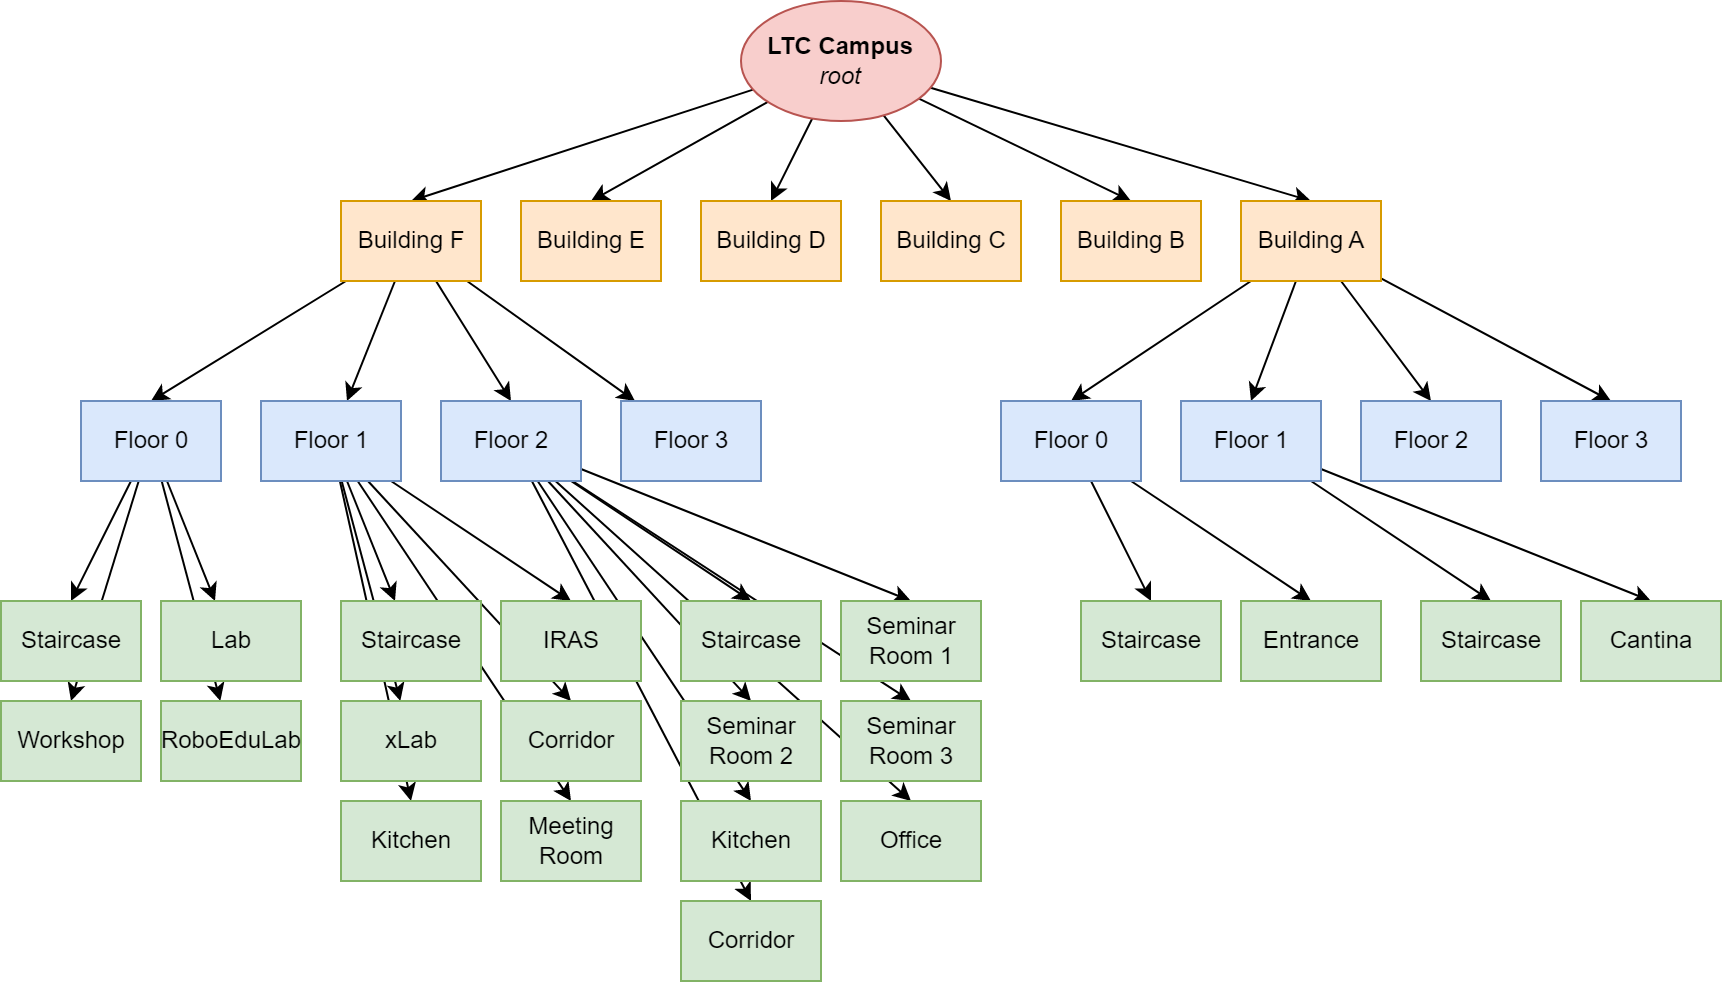
\includegraphics[width=\textwidth]{figures/20_state_of_the_art/hierarchical_graph.png}
    \caption[Representation of the structure of an H-Graph as tree]{Representation of the structure of an H-Graph with three hierarchical layers as a tree with depth of three. This example shows the whole campus on layer 0 (red), the buildings of this campus on layer 1 (orange), the floors of each building on layer 2 (blue) and the single rooms on layer 3 (green). For better visibility only some example nodes are fully expanded}
    \label{fig:h_graph}
\end{figure}

For use in navigation the structure of the \gls{h_graph} represents the physical environment, this was first applied to mobile robot path planning by \cite{fernandez_hierarchical_1998} \cite{fernandez-madrigal_multi-hierarchical_2001}. The nodes in each graph are connected only if a drivable connection between these buildings or rooms exits. To make this space plannable the connection has a cost corresponding to the shortest path distance between these two entities. This allows a common graph solver algorithm like Dijkstra or A* to find the shortest path in each graph. The advantage of a \gls{h_graph} is that not every leaf node in the tree has to be searched because only the nodes which are on the path of the higher layer are relevant. This reduces the search space and the time needed to find the optimal path in large environments drastically. To combine a feasible path from all different graphs on the lowest layer, continuity between paths of different subgraphs has to be ensured.

One proposed solution is the Hierarchical D* (HD*) algorithm from Cagigas \cite{cagigas_hierarchical_2005}. Cagigas breaks down an environment by hierarchical decomposition into an \gls{h_graph}. In each subgraph the shortest connections to elevators are precalculated and stored as weight of the connection in the meta-graph. This is called materialization of costs. After finding the shortest path based on these costs, a reconstruction process is applied that links the obtained partial paths. Cagigas extends the original D* algorithm \cite{hebert_optimal_1997} for this hierarchical planning. The D* algorithm is represents a dynamic or on-line version of the A* algorithm. The D* reuses and updates the calculated cost from the intial search to replan the path if an dynamic obstacle blocks the initial path. This is an efficient way to replan without calculating all costs again. Cagigas defines three types of hierarchical path planning: 
\begin{enumerate}
    \item \textbf{Horizontal path planning (HPP):} paths between nodes connected in a horizontal way. Equivalent to traditional robot path planning.
    \item \textbf{Vertical path planning (VPP):} paths between nodes connected in a vertical way. Namely, paths that begin on a floor and finish on another floor of the same building.
    \item \textbf{Inter-building path planning (IPP):} paths between nodes of different buildings. These paths begin on a floor of a building and finish on a floor of another building.
\end{enumerate}
Cagigas identifies the elevator selection problem shown in Figure \ref{fig:elevator_selection_problem} which occures in vertical path planning. The benefits of the HD* can not be applied here and a complete path replanning is necessary.

\begin{figure}[h]
    \centering
    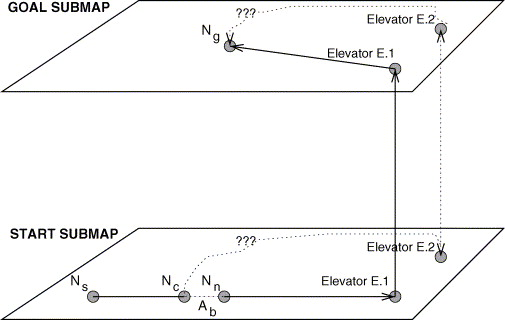
\includegraphics[width=0.75\textwidth]{figures/20_state_of_the_art/elevator_selection_problem.jpg}
    \caption[The elevator selection problem]{On-line vertical path planning. A “broken” arc \(A_b\) (obstacle) is detected between the current node \(N_c\) and the next node \(N_n\) in an initial path that joins a start node \(N_s\) and a goal node \(N_g\). The path planner module has to select an elevator entrance and there are two possibilities: the elevator entrance in the initial path (Elevator E.1) or an alternative elevator entrance (Elevator E.2). This last selection implies a complete path replanning. (Source: \cite{cagigas_hierarchical_2005})}
    \label{fig:elevator_selection_problem}
\end{figure}


In \cite{seder_hierarchical_2011} Seder proposed the Focussed Hierarchical D* (FHD*) algorithm. It improves the HD* algorithm by Cagigas in the following points:
\begin{enumerate}
    \item optimal placement of the so-called bridge nodes needed for hierarchy creation.
    \item focusing the search around the optimal path, which reduces the search area without loss of optimality.
    \item introduction of partial starts and partial goals, which further reduce computational time of replanning operations.
\end{enumerate}

Especially the optimal placement of bridge points is important to ensure optimal paths over multiple hierarchies. Bridge nodes are be placed at the optimal path that is to be followed by a mobile robot on its way from one room to the other. Seder calculates the optimal position by using a safety cost mask to find the middle point in a narrow passage. This corresponds to the safest point for a robot to drive through a door. In Figure \ref{fig:bridge_node_placement} an example of the bridge node placement can be seen. Seder shows, that the FHD* agorithm is faster during replanning, needs fewer iterations and fewer explored nodes compared to the D*, FD* and HD* algorithms.

\begin{figure}[h]
    \centering
    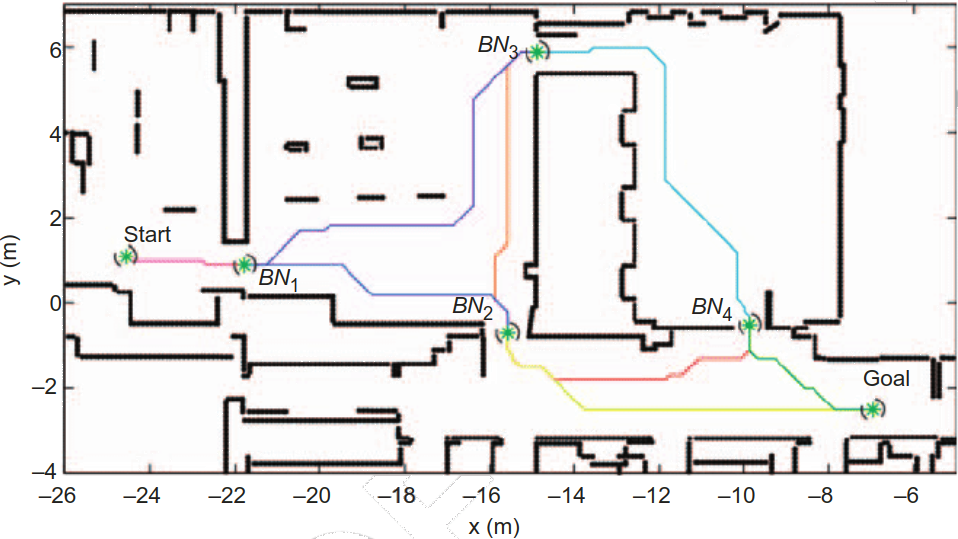
\includegraphics[width=0.75\textwidth]{figures/20_state_of_the_art/bridge_node_placement_paths.png}
    \caption[The bridge nodes with precalculated paths]{The bridge nodes BN 1-4 and the precalculated paths between them. (Source: \cite{seder_hierarchical_2011})}
    \label{fig:bridge_node_placement}
\end{figure}

Gregoric \cite{gregoric_autonomous_2022} further extends the ideas of Seder by using the E* algorithm \cite{philippsen_interpolated_2005}. This leverages the A* to plan with an arbitrary angle instead of a fixed grid with 90 degrees (4 neighbours) or 45 degrees (8 neighbours). Gregoric proposes a method to automatically generate an H-Graph from CAD floor plans. On floor map level this is done by using the safety cost mask. Connections between buildings are assumed to be on the ground floor. Vertical bridge connections are found with three conditions: 

\begin{enumerate}
    \item Comparing the positions of nodes on each floor
    \item The size of the room 
    \item The number of doors connecting this room to others
\end{enumerate}

Ryu uses a different approach in generation of the \gls{h_graph} as well as finding the subpaths \cite{ryu_hierarchical_2020}. Ryu only uses a two-layered hierarchy on a single floor. The two hierarchies are the so called inter- and intra-regional graphs which correspond to the connections between rooms and the path between the doors in each room. The hierarchy is automatically created by segmenting the entire floor plan into rooms. This is done by using the marker controlled watershed algorithm \cite{parvati_image_2009}. 

\begin{figure}[h]
    \centering
    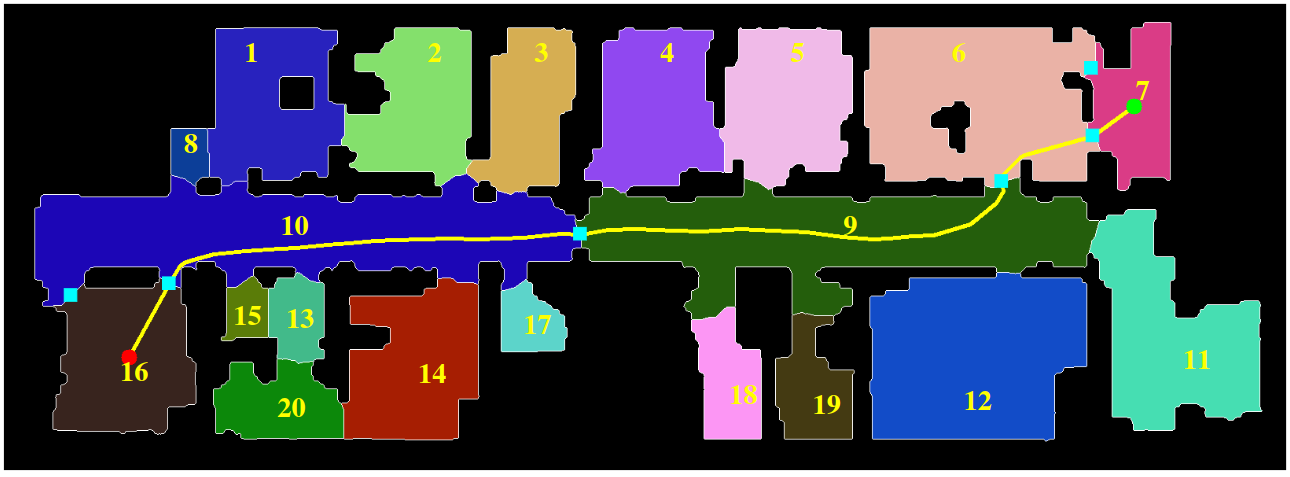
\includegraphics[width=0.75\textwidth]{figures/20_state_of_the_art/ryu_floor_path.png}
    \caption[The segmented floor map with combined inter-regional paths]{The segmented floor map with combined inter-regional paths (Source: \cite{ryu_hierarchical_2020})}
    \label{fig:ryu_floor_path}
\end{figure}

For the next step Ryu proposes an algorithm for detecting safe junction nodes as bridge between each room. A distance transform is used and the node with the highest clearance to the obstacle is chosen. This is similar to the process from Seder where a safety cost mask is applied. With these junction nodes the intra-graph is created as seen in Figure \ref{fig:ryu_floor_path}. Ryu then uses a Skeletonization-Informed Rapidly Exploring Random Tree* (SIRRT*) to plan the inter-regional path. This is an extension from the classic sample-based RRT algorithm. It uses a skeletonized representation of the grid map of a single room. This skeleton is used to inform the sampling of the RRT algorithm by generating nodes close to the skeleton. In Figure \ref{fig:ryu_sirrt} a solution path of the SIRRT* is shown. 

\begin{figure}[h]
    \centering
    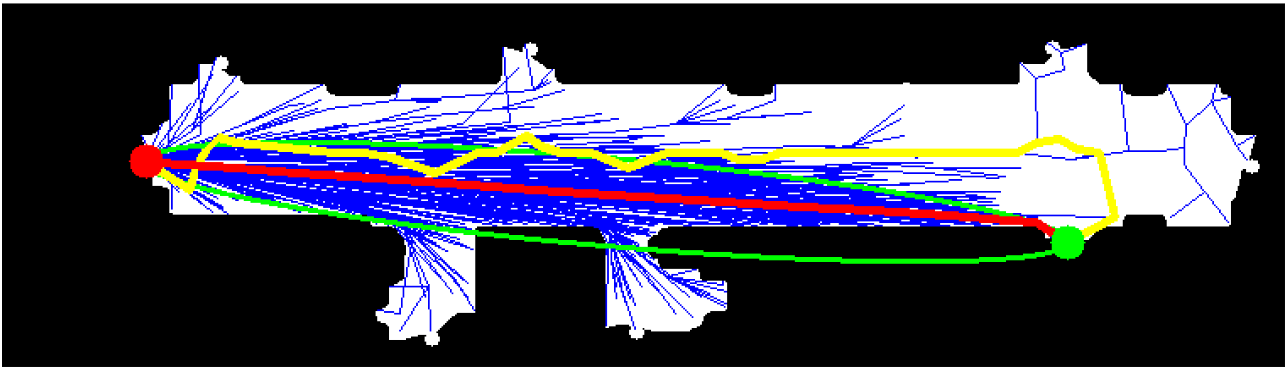
\includegraphics[width=0.75\textwidth]{figures/20_state_of_the_art/ryu_sirrt.png}
    \caption[Path planning with the SIRRT*]{An example of local path-planning for Segment “9” using the skeletonization informed rapidly exploring random tree* (SIRRT*): The red dot is the start position; the green dot is the goal. The initial skeleton path (yellow line). The final tree (blue line) and the optimized path (red line). The are for generating new sample nodes (green) (Source: \cite{ryu_hierarchical_2020})}
    \label{fig:ryu_sirrt}
\end{figure}

The previous papers were using simulated 2D gridmap environments. They have not mentioned the application on a real robot. Dihman et al \cite{dhiman_ros_2020} and Wang et al \cite{wang_autonomous_2019} separately introduced a framework for using multi-floor navigation with ROS 1 on a real robot. Wang uses a modified A* algorithm to plan paths that are more centered in the hallway. The main contribution is the development of an CNN to detect the current floor by pictures. A VGG16 network architecture is trained with 7,000 images to predict the current floor of the robot. It is not mentioned if automatic hierarchy creation or an H-Graph is used for navigation. It is also not mentioned how the robot knows which elevator or floors it needs to drive to. Only on floor map level path planning is done with the extended A*. Wang uses a real robot, the Pioneer 3-DX, and integrates everything in the existing ROS navigation stack. Dihman in comparison proposes a method for global path planning on a cost graph. This is one single graph to represent the floors and rooms of a single building, see Figure \ref{fig:dihman_cost_graph}. Vertical connections are drawn in the same graph and represented with corresponding traversal costs. Dihman also modifies the existing ROS 1 navigation stack to account for multiple robots and autonomous exploration. Additionally the map server is extended for a multi-level occupancy gridmap and the global planner plans with respect to the cost graph.

\begin{figure}[h]
    \centering
    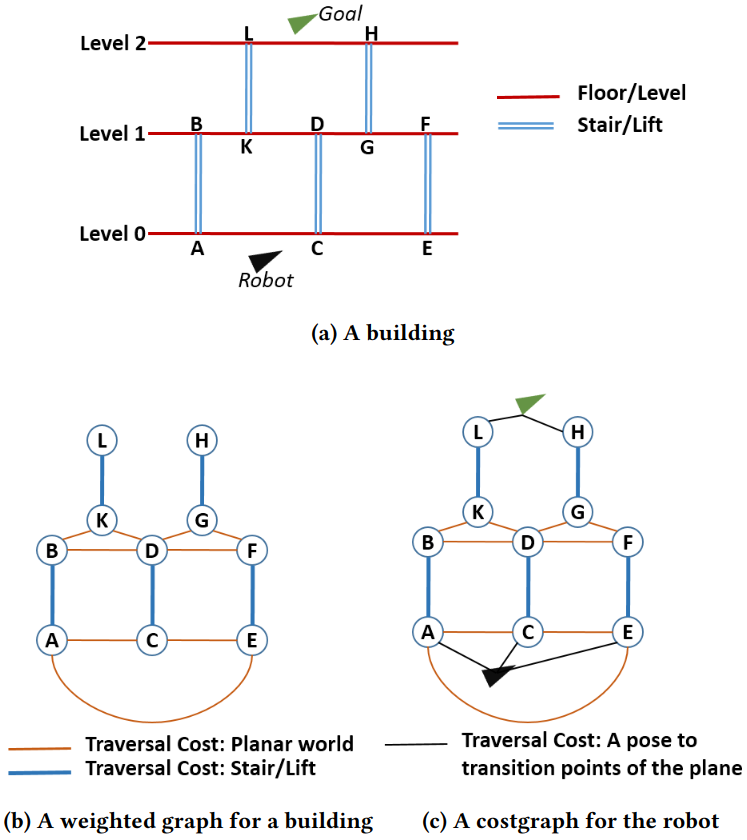
\includegraphics[width=0.75\textwidth]{figures/20_state_of_the_art/dihman_cost_graph.png}
    \caption[The costgraph for the robot]{(a) A building is represented as levels with stair or lift connection between floors, represented by thick blue parallel-lines. Blue and green color triangle represent current robot pose and goal pose respectively. (b) The building is transformed into a weighted graph. The node names refer to connection between the floor. (c) represents a weighted graph which includes edges from current robot pose and goal pose to the conncetion on the respective floor. This graph will be further used for solving global path planning. (Source: \cite{dhiman_ros_2020})}
    \label{fig:dihman_cost_graph}
\end{figure}

A comparison of these approaches to hierachical path planning in multi-floor environments is done in Chapter \ref{sec:research_gap}.
It can be seen, that the focus is either on the automatic hierarchy creation and efficient replanning or on the integration with ROS and the extension with additional features like CNN floor detection or multiple robots. This work aims to provide a mixture of these features by providing a method for automatic hierarchy creation for an H-Graph and integrating it in the new ROS 2 in simulation and for a real robot.

%% ==============================
\section{Straight Path Planning}
\label{sec:straight_paths}
%% ==============================

\begin{enumerate}
    \item Voronoi Diagrams, EVG (with sensory horizont)
    \item Smoothing algorithms (Bezier curves, B-Splines, Bechtold and Glavina, Latombe)
    \item ROS2 OpenRMF
    \item Paper Straight Skeleton Based Automatic Generation of Hierarchical Topological Map in Indoor Environment
    \item Semantic and Topological Mapping using Intersection Identification (Has comparison on the AWS hospital map!)
\end{enumerate}

In this section the recent approaches to straight path planning are presented. This gives an overview of the relevant existing works corresponding to the second research question: "How to plan paths that are straight and human-predictable?"

A common approach in path planning is the creation of a roadmap. The advantages of roadmaps are that they are very efficient for replanning because the roadmap is not recalculated every time. Depending on the creation process roadmaps do not guarantee optimality but they provide a feasible answer within a short period of time. This is especially useful for motion planning in a higher dimension space for multi axis manipulators. The configuration space \(C\) in the case of plane 2D path planning has the same x and y axis as the real space. Obstacles in \(C\)-space are inflated by the size of the robot to find collision free paths.

\begin{displayquote}
    \enquote{The roadmap approach to path planning consists of capturing the connectivity of the robot's free space in a network of one-dimensional curves, called the roadmap, lying in the free space \(C_{free}\) or its closure \(cl(C_{free})\). Once a roadmap \(R\) has been constructed . it is used as a set of standardized paths. Path planning is thus reduced to connecting the initial and goal configurations to points in \(R\) and searching \(R\) for a path between these points. The constructed path, if any, is the concatenation of three subpaths: a subpath connecting the initial configuration to the roadmap, a subpath contained in the roadmap, and a subpath connecting the roadmap to the goal configuration.} \cite{latombe_robot_2003}
\end{displayquote}

In the previously presented RRT or PRM algorithm the roadmap is created by randomly sampling free points in \(C\)-space and connection them with a collision free egde. Another approach for roadmap creation is the Voronoi diagramm. The diagram is the set of all points with the largest distance to neighbouring obstacles. It consits of free paths which maximize the obstacle clearance.

\begin{figure}[h]
    \centering
    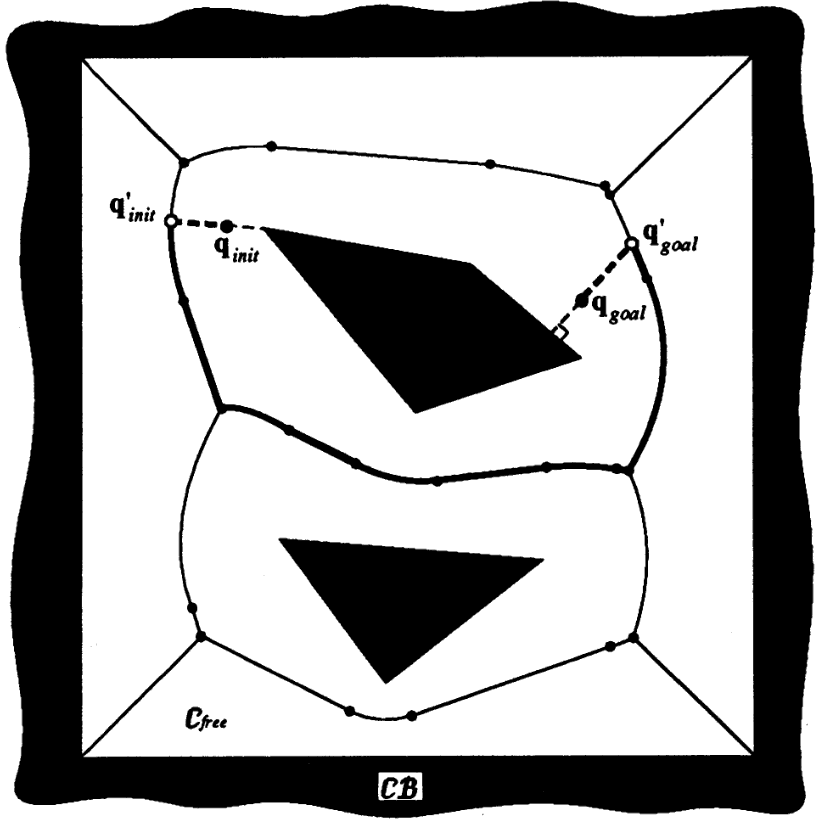
\includegraphics[width=0.5\textwidth]{figures/20_state_of_the_art/voronoi_diagram.png}
    \caption[The Voronoi diagram]{This figure shows the Voronoi diagram in a configuration space with a polygonal \(C\)-obstacle region. The free space is externally bounded by a rectangle. The initial and goal configurations \(q_{init}\) and \(q_{goal}\) are mapped into the Voronoi diagram to \(q'_{init}\) and \(q'_{goal}\), each by drawing the line along which its distance to the boundary to the \(C\)-obstacle region increases the fastest. (Source: \cite{latombe_robot_2003})}
    \label{fig:voronoi_diagram}
\end{figure}

The generalized Voronoi diagram, also called graph (GVG / GVD) is defined as the one-dimensional set of points equidistant to n or more obstacles in n-dimensions. By pruning the graph based on a minimum length the reduced generalized Voronoi graph (RGVG) can be obtained. Beeson et al. \cite{beeson_towards_2005} extended the GVD to solve a limited sensory horizont of mobile robots. The Extended Voronoi graph (EVG) transitions from a midleline in narrow corridors to a line which follows the walls in open rooms.  However the resulting paths suffer from noise in the measurements resulting in not straight paths. Also in junctions the GVD and EVG produce paths that bend into the intersections open space. Thus creating a unnecessary curve for the straight direction as seen in Figure \ref{fig:htm_path_comparison} c).

\begin{figure}[h]
    \centering
    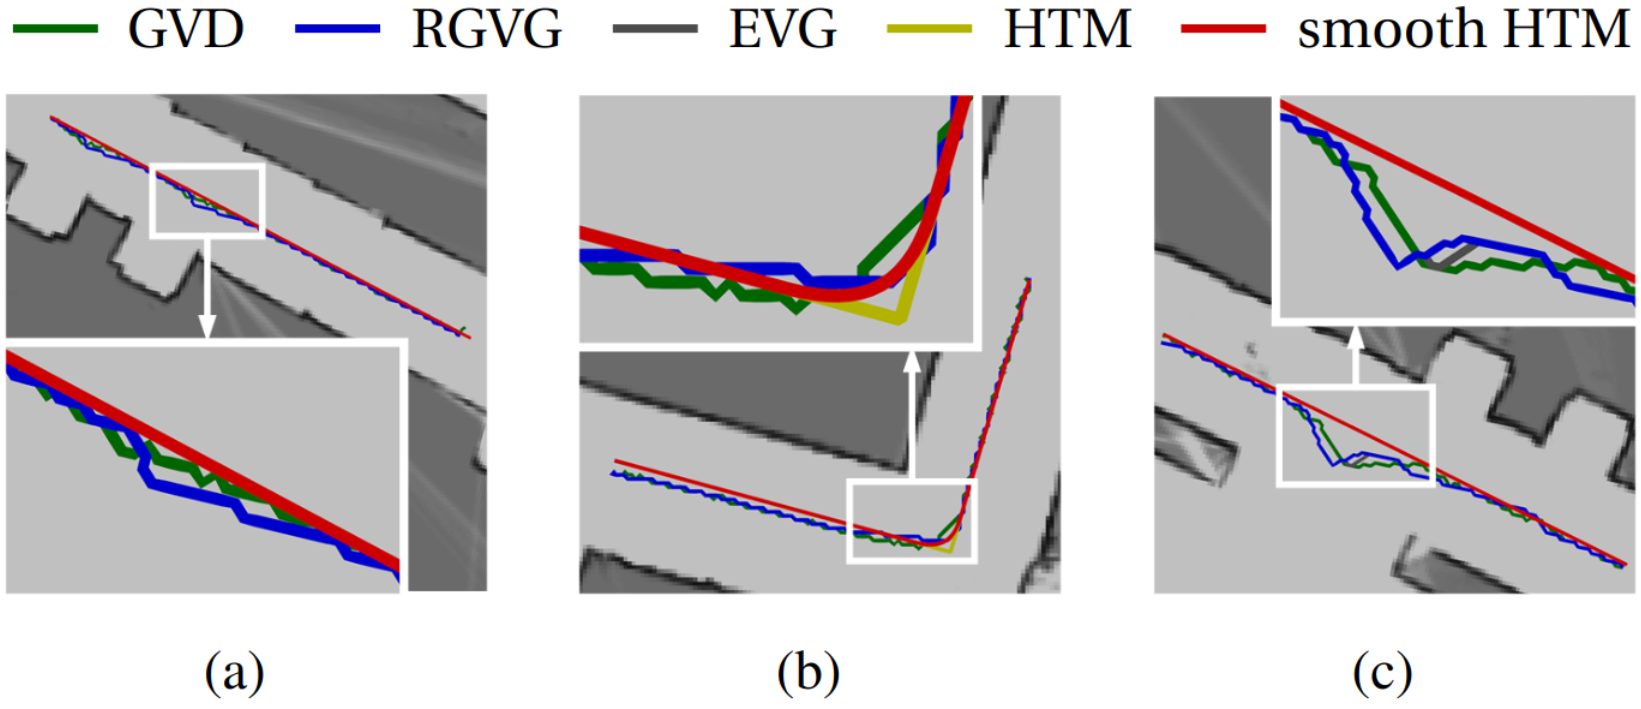
\includegraphics[width=0.75\textwidth]{figures/20_state_of_the_art/htm_path_comparison.png}
    \caption[Comparison between straight paths]{EVG based tracks coincide with RGVG based tracks within the sensory horizon. HTM based tracks coincide with smooth HTM when non-turning. (a) Tracks in the straight corridor. (b) Tracks in the turning corridor. (c) Tracks in the corridor with a room on the side. (Source: \cite{hou_straight_2021})}
    \label{fig:htm_path_comparison}
\end{figure}

Another approach for retrieving the topological map of an environment is the Straight Skeleton \cite{maurer_novel_1996}. In comparison to Voronoi diagrams this method does not use a distance function but shrinks the obstacle-polygon into the free space. Each edge is moved along its normal axis at the same speed, this creates a boundary where the shrinked edges touch. Based on this Straight Skeleton Hou et al. \cite{hou_straight_2021} improved the straight path generation and counters the jitter problem of the EVG. Hou et al. proposes the Hierarchical Topological Map (HTM) for the automatic generation of valid straight paths. The hierarchical approach first generates the straight skeleton and then detects intersections or small rooms where the jitter problem occures. These sections are extracted and a separate skeleton is generated inside which is then connected back to the global path. Finally a clothoid-based smoothing method is applied to ensure the curvature continuity of generated tracks. A comparison of the discussed algorithms for generating topological maps and straight paths can bee seen in Figure \ref{fig:htm_global_comparison}

\begin{figure}[h]
    \centering
    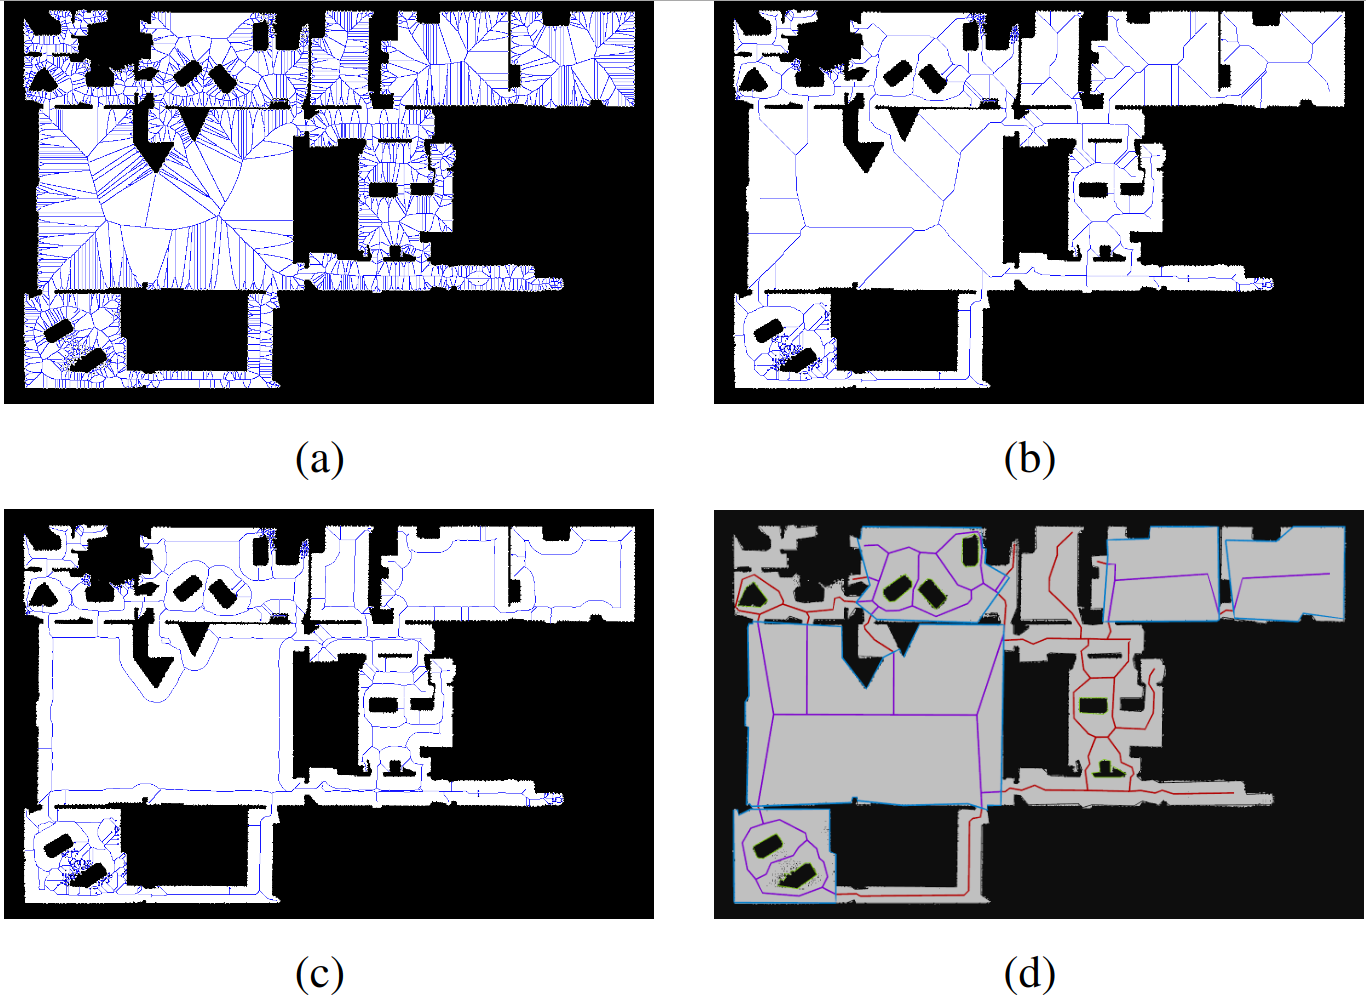
\includegraphics[width=\textwidth]{figures/20_state_of_the_art/htm_global_comparison.png}
    \caption[Comparison of generated topological maps]{Comparison of skeleton generation, using the grid map obtained from \cite{beeson_towards_2005}. (a) GVD. (b) RGVG. (c) EVG with a sensory horizon of 1.25m. (d) HTM. Primary tracks, secondary tracks, and regions are marked in red, purple, and blue, respectively. (Source: \cite{hou_straight_2021})}
    \label{fig:htm_global_comparison}
\end{figure}

The presented methods focus on the goal of extracting a topological map from the gridmap. The HTM also focuses on generating paths that a straight. Further discussion on the limitations of these approaches and the resulting research gap this work aims to address is done in Chapter \ref{sec:research_gap}. 

%% ==============================
\section{Research Gap}
\label{sec:research_gap}
%% ==============================

Research gap from previous approaches:
\begin{enumerate}
    \item Hierarchical graphs are not per room or per floor which makes it difficult to append slamed maps or semantic information
    \item Hierarchical graphs are not used in ROS2 Nav Stack
    \item Approaches for straight paths are not deterministic and not human-predictable
    \item Approaches for straight paths are not implemented in ROS2 Nav Stack
    \item Approaches for straight paths only work well in small corridors
\end{enumerate}

In Table \ref{tab:overview_q1} an overview on the state of the art to research Question 1: "How to navigate in complex multi-floor environments?" is given. The different approaches to hierarchical path planning are presented in Chapter \ref{sec:hierarchical_planning}, this Chapter discusses the limitations of these methods and shows the research gap for this work.

\begin{table}[]
\centering
\caption{Overview on the state of the art in hierarchical path planning}
\label{tab:overview_q1}
\resizebox{\textwidth}{!}{%
\begin{tabular}{@{}llllllll@{}}
\toprule
\textbf{Key topics} & \multicolumn{1}{c}{\textbf{\begin{tabular}[c]{@{}c@{}}Cagigas\\2005 \cite{cagigas_hierarchical_2005}\end{tabular}}} & \multicolumn{1}{c}{\textbf{\begin{tabular}[c]{@{}c@{}}Seder\\2011 \cite{seder_hierarchical_2011}\end{tabular}}} & \multicolumn{1}{c}{\textbf{\begin{tabular}[c]{@{}c@{}}Gregoric\\2022 \cite{gregoric_autonomous_2022}\end{tabular}}} & \multicolumn{1}{c}{\textbf{\begin{tabular}[c]{@{}c@{}}Ryu\\2020 \cite{ryu_hierarchical_2020}\end{tabular}}} & \multicolumn{1}{c}{\textbf{\begin{tabular}[c]{@{}c@{}}Wang\\2019 \cite{wang_autonomous_2019}\end{tabular}}} & \multicolumn{1}{c}{\textbf{\begin{tabular}[c]{@{}c@{}}Dihman\\2020 \cite{dhiman_ros_2020}\end{tabular}}} & \multicolumn{1}{c}{\textbf{\begin{tabular}[c]{@{}c@{}}{[}This work{]}\\2023\end{tabular}}} \\ \midrule
\begin{tabular}[c]{@{}l@{}}Path planning\\ algorithm\end{tabular} & HD* & FHD* & E* & SIRRT* & A*' & \begin{tabular}[c]{@{}l@{}}? /\\ Dijkstra\end{tabular} & \begin{tabular}[c]{@{}l@{}}ILIR /\\ Dijkstra\end{tabular} \\
\smallskip \\
\begin{tabular}[c]{@{}l@{}}Efficient on-line\\ replanning\end{tabular} & Yes & Yes & Yes & No & No & No & Yes \\
\smallskip \\
Map source & 2D Sim & 2D Sim & \begin{tabular}[c]{@{}l@{}}Floor\\ plans\end{tabular} & SLAM & SLAM & \begin{tabular}[c]{@{}l@{}}SLAM\\ Multi-robot\end{tabular} & SLAM \\
\begin{tabular}[c]{@{}l@{}}Hierarchy\\ creation\end{tabular} & Manual & \begin{tabular}[c]{@{}l@{}}Safety\\ cost mask\end{tabular} & \begin{tabular}[c]{@{}l@{}}Safety\\ cost mask,\\ matching\end{tabular} & \begin{tabular}[c]{@{}l@{}}Water-\\ shed\end{tabular} & \begin{tabular}[c]{@{}l@{}}CNN floor\\ detection\end{tabular} & Manual & Watershed \\
\smallskip \\
Hierarchy levels & 3 & 2 & 4+ & 2 & 3 & 3 & 4+ \\
\smallskip \\
\begin{tabular}[c]{@{}l@{}}Implementation\\ on real robot\end{tabular} & - & - & - & - & ROS 1 & ROS 1 & ROS 2 \\ \bottomrule
\end{tabular}%
}
\end{table}

The earlier work of Cagigas and Seder focuses on solving the planning problem as a whole. They develop one planner which solves the global path through the hierarchy as well as the path on the lowest gridmap level. Additionally they use a D* algorithm which is very efficient for replanning when obstacles are detected. This approach results from the fact, that to this time no open source framework for path planning, like ROS, existed. This required to solve most robotic problems from the ground up. With the widespread distribution of ROS many open source implementations for common planners exist. This has the advantage of profiting from efficiently implemented planners in an integrated framework and allows to focus on developing just the missing part. This development is seen with Wang and Dihman, as both use ROS 1 and don't implement the basic planners themselves. The disadvantage is that solution for the entire problem of hierarchy solving and path planning combined could be more efficient. However reusability and community-defined interfaces enable the fast development in robotics research and thus building upon existing software is currently preferred. The analysis of available literature shows that with the tools of ROS 2 no such open-source solution exists. The goal of this work is to develop a hierarchical path planner by using the existing frame work of ROS 2 and Nav2. Additionally the proposed straight roadmap on the lowest level allows for efficient replanning.

Gregoric uses the path planning ideas from Seder and focuses on automatic generation a hierarchical graph of the environment from floor plans. This extends the previous approaches as the number of levels are theoretically infinite. Although automatic hierarchy creation is only shown for room segmentation and floor matching. Additionally a very simple multi-building environment is assumed, where vertical bridge nodes are always directly above each other and connect only floors of the same building. Further buildings are assumed to have only one connection between each other on the ground floor. Although in complex environments bridges on upper floors, ramps or densely connected building sections are possible. Ryu in comparison only focuses on hierarchy creation for two levels but proposes a new method for automatic room segmentation from SLAMed gridmaps. The goal of this work is leveraging the ideas of Gregoric of n-level hierarchies for complex environments with arbitrary connections and using the approach from Ryu for automatic room segmentation. As both works have not been implemented an a real robot or are available as open-source, the developed algorithms should be easy to use on a real mobile robot with ROS 2.

For the problem of straight path planning, an comparison of existing approaches can be seen in Figure \ref{fig:htm_global_comparison}. Only Hou focuses on creating straight paths, the most common approach for a straight indoor roadmap is manual waypoint selection. One promising tool for that is OpenRMF from OpenRobotics \cite{openrobotics_open-rmf_2023} which is currently in development. The aim of this tool is mainly fleet management and interoperability between robot vendors but it also uses a roadmap of preplanned straight paths. There is currently no plan to generate these straight paths automatically. For real production environments this is due to safety reasons. However if there would be a tool which initially proposes straight paths that can be refined by manually moving specific waypoints it would reduce the time for implementation drastically. The goal of this work is develop such an algorithm for an initial straight roadmap.

The HTM approach from Hou generates mostly paths that a straight. This makes these paths predictable for humans walking in the same area as the mobile robot. Also all of these approaches are deterministic. This means, given the same gridmap, these algorithms always produce the same output path. There is not a probabilistic function involved which generates random points like in the RRT or PRM. A path that is deterministic is also more predictable for humans as the robot behaves the same. The advantage is that humans working in the same space can learn the paths of the mobile robot and can predict areas where a robot might drive through. This is useful for the hospital environment of the PeTRA use-case. However the generated paths or not ideal for open spaces and large rooms as seen in Figure \ref{fig:htm_global_comparison} d). Assuming this is a lobby or other large room where people might wait and walk between doors. The path generated by the HTM are not intuitive. One would expect a robot to drive in a straight path parallel to the wall and not in a triangle shape driving at an angle and then returning to the same wall again. This requires a metric for the quality of the straight paths and to measure the effect of disturbing the public space used by other people. This work compares the proposed roadmap planner against other approaches and proposes a metric for the disturbance of public space.

In general this research field is not very active. There are a few algorithms and limited proof of concept implementations but there is a lack for a solution of the problem in its entirety. In particular a comprehensive benchmark environment for multi-floor scenarios is needed to test and compare methods with other researchers. Additionally the hierarchy creation for a large, complex environment is a slow and manual process which is not completely solved yet. Both of these problems are out of scope for this work, but once solved could pave the way for the easy commission of large fleets of robots in a multi-floor building. In context of the increasing number of tasks that can be automated with the advanced capabilities of AI and scene understanding more and more service tasks could be carried out by mobile robots.